\section{Overview of population forecasting methods}

Population forecasting is the practice of predicting future population sizes and structures based on current demographic data, trends, and assumptions regarding factors like fertility rates, mortality rates, and migration flows. These forecasts are crucial for policymakers, urban planners, and organizations in planning for future needs in healthcare, education, infrastructure, housing, and employment. By understanding potential population shifts, governments can allocate resources effectively and prepare for aging populations, urban growth, or potential labor shortages.

An essential tool that underpins population forecasting is the population census. A census is a systematic effort to collect detailed information about every individual within a country or region, including data on age, sex, race, education, employment, and living conditions. Conducted typically every 10 years, censuses provide a comprehensive snapshot of a population at a specific moment in time. This data is not only crucial for immediate decision-making but also serves as the foundation for future demographic analysis and projections. Without accurate and timely census data, population forecasts would lack a reliable baseline, making predictions about future demographic changes significantly less accurate.

Censuses have a long history, dating back to ancient civilizations like Egypt and Rome, where they were used primarily for taxation and military conscription purposes. The modern concept of the census, however, began in Sweden in 1749 and spread to other European countries in the centuries that followed \cite{BirthOfModernCensusInSweden}. In the United States, the first national census was conducted in 1790 and has been carried out every decade since, even helping other countries around the world conduct their own censuses \cite{UsaHelpingOthersWithCensuses}. Over time, census methods have evolved from basic headcounts to more sophisticated surveys, incorporating data collection techniques that include digital tools, administrative records, and statistical sampling.

Censuses are typically conducted through a combination of self-reporting by households, in-person interviews, and administrative record analysis. The process generally starts with extensive planning and public outreach to ensure high participation rates. Census workers are employed to visit households and collect data either through interviews or by delivering and retrieving census forms. In many countries, individuals are encouraged to complete the census forms online or via mail, offering a more efficient and cost-effective method of data collection. The forms usually cover essential demographic details such as age, sex, household size, educational attainment, occupation, and housing characteristics. Modern censuses are increasingly utilizing digital tools and new technologies to streamline the collection and processing of data, helping governments to obtain more accurate and timely population information \cite{CensusPrinciplesAndRecommendations}.

The most recent 2020 round of population censuses was a global effort where many countries conducted their censuses, despite facing significant challenges due to the COVID-19 pandemic \cite{Codid19ImplicationsOnCensusConduct}. The pandemic disrupted traditional census operations, leading to delays, changes in methodology, and increased reliance on digital and administrative data collection methods. Some countries moved more census processes online to reduce in-person contact, while some, postponed their census altogether. The 2020 round highlighted the growing importance of digital tools, remote data collection, and administrative records in ensuring accurate population counts during unforeseen circumstances.

\begin{figure}[H]
    \centering
    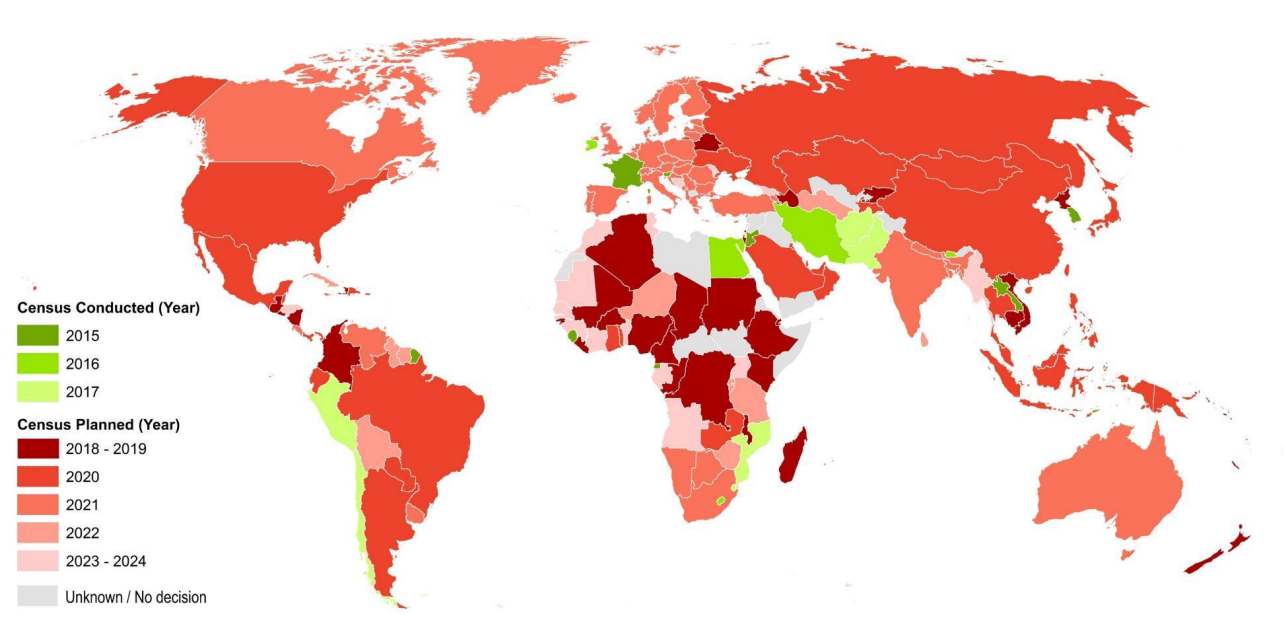
\includegraphics[scale=0.5]{images/most-recent-census-conducting-year-world-map.png}
    \caption{National dates for 2020 round of population census \cite{WorldMapOf2020RoundCensus}}
    \label{img:most-recent-census-conducting-year-world-map}
\end{figure}

With this information about the general population census conduct it is now possible to dive deeper in to the most popular census methods currently used around the world - self-reporting method, interview method and population registry analysis method with an additional alternative population census method offered and analysed.